\section{Data transmission comparison}

We next evaluate the time it took both implementations to transmit the aforementioned MQTT messages.
To do so, we have used the previously described methodology.
That is, we have transmitted the MQTT messages shown in~\ref{appendix:mqtt_message} for their respective scenario and have measured the total time taken for the transmission to occur.

Figure~\ref{fig:comm_time_home} shows the results for the data transmission in the IoT home scenario.
We can see that MQuicTT performs comparably to the base $rumqtt$ implementation.
$MQuicTT$ performs better in the cases of 3g, 4g and WiFi, and loses out to the base implementation in Zigbee and ethernet.
The difference however is not substantial and we can see from the variance that the implementations are comparable in performance.
Notably, $MQuicTT$ experiences higher variance which may imply that it is more affected by changes in the simulation environment between tests, while the base implementation is more consistent.
Overall, in this scenario, $MQuicTT$ performs on par with the TCP implementation, however it also presents no advantage in terms of performance.

\begin{figure}
    \centering
    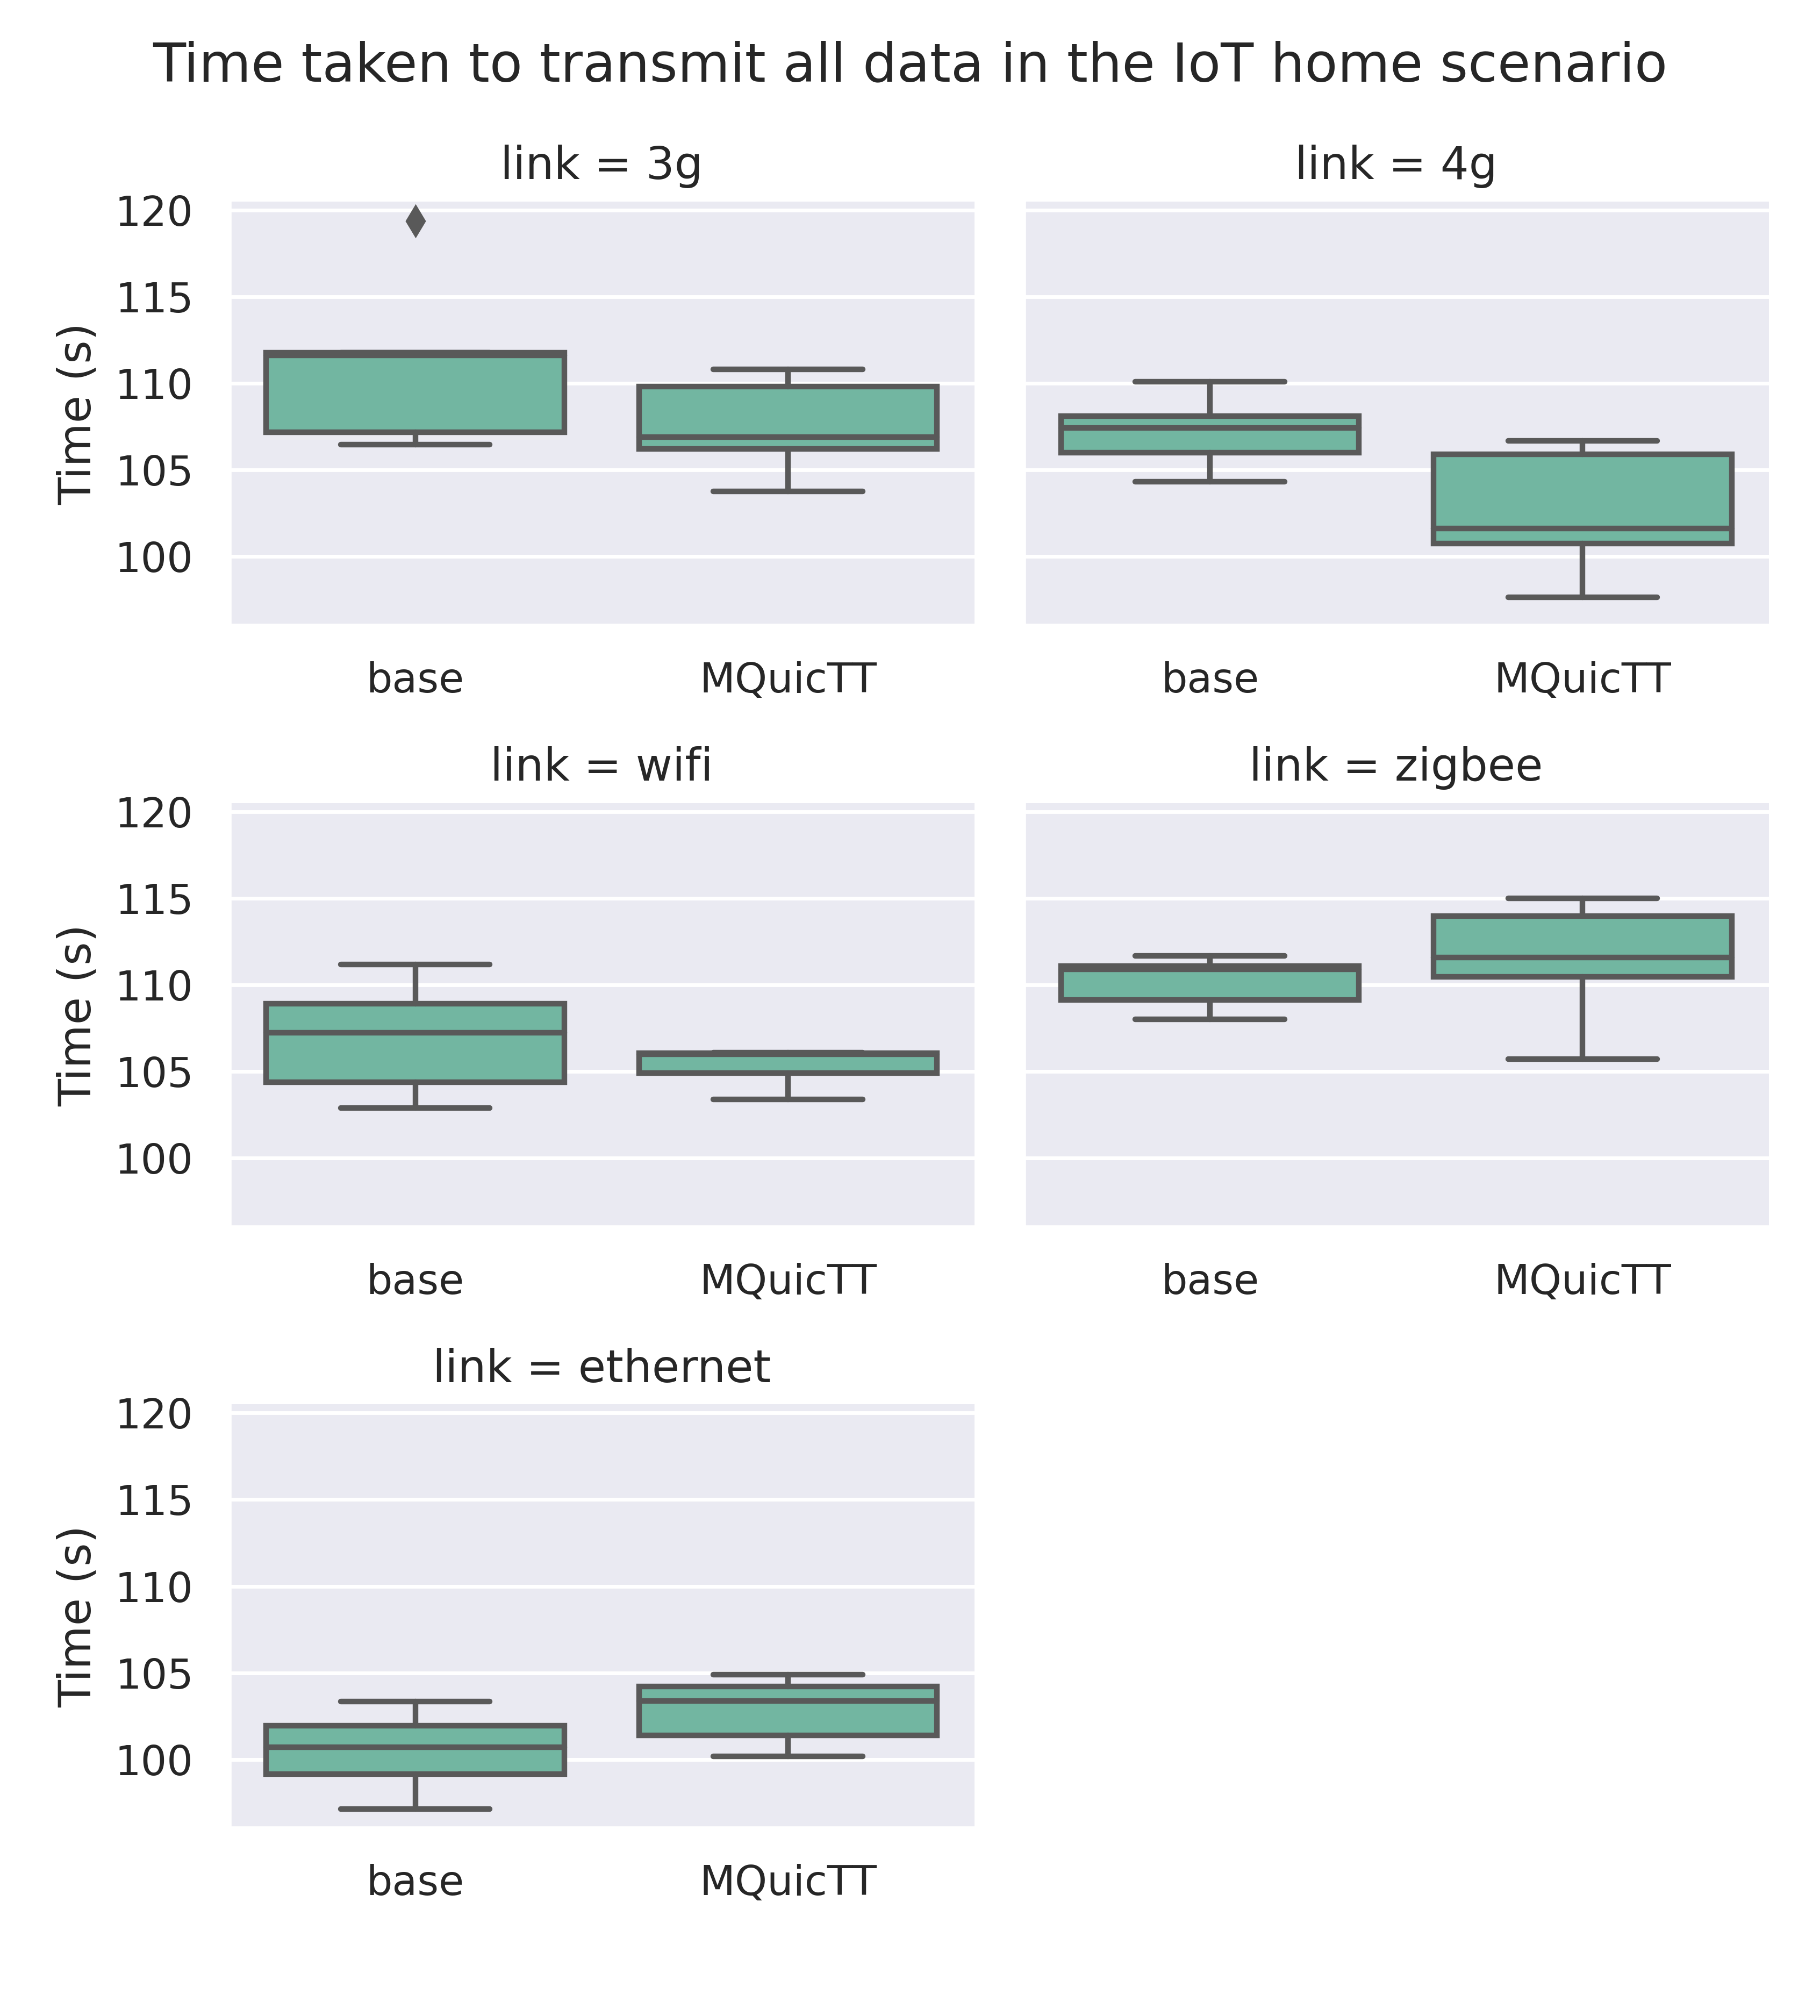
\includegraphics[width=1\linewidth]{images/analysis_comm_time_home.png}
    \caption{The time it took for the implementations to transmit the MQTT messages in the IoT home scenario.
        The time for each plot   is shown in seconds.
        We can see that MQuicTT experiences higher variance, but performs on par with the base implementation overall.}
    \label{fig:comm_time_home}
\end{figure}

Figure~\ref{fig:comm_time_farm} shows the results for the printer farm scenario.
As previously discussed, this scenario presents higher packet loss to simulate the kind of congestion a link may experience in an industrial IoT application.
From the results we can see that $MQuicTT$ again performs on par with the base implementation.
We can also see that $MQuicTT$ experiences more variance in this scenario too.
The theoretical advantage that the QUIC protocol may provide in environments with high packet loss does not seem to be demonstrated in this scenario.
This is perhaps due to the packet loss not being extreme enough for QUIC to show advantage.
Overall, the implementations again perform comparably.

\begin{figure}
    \centering
    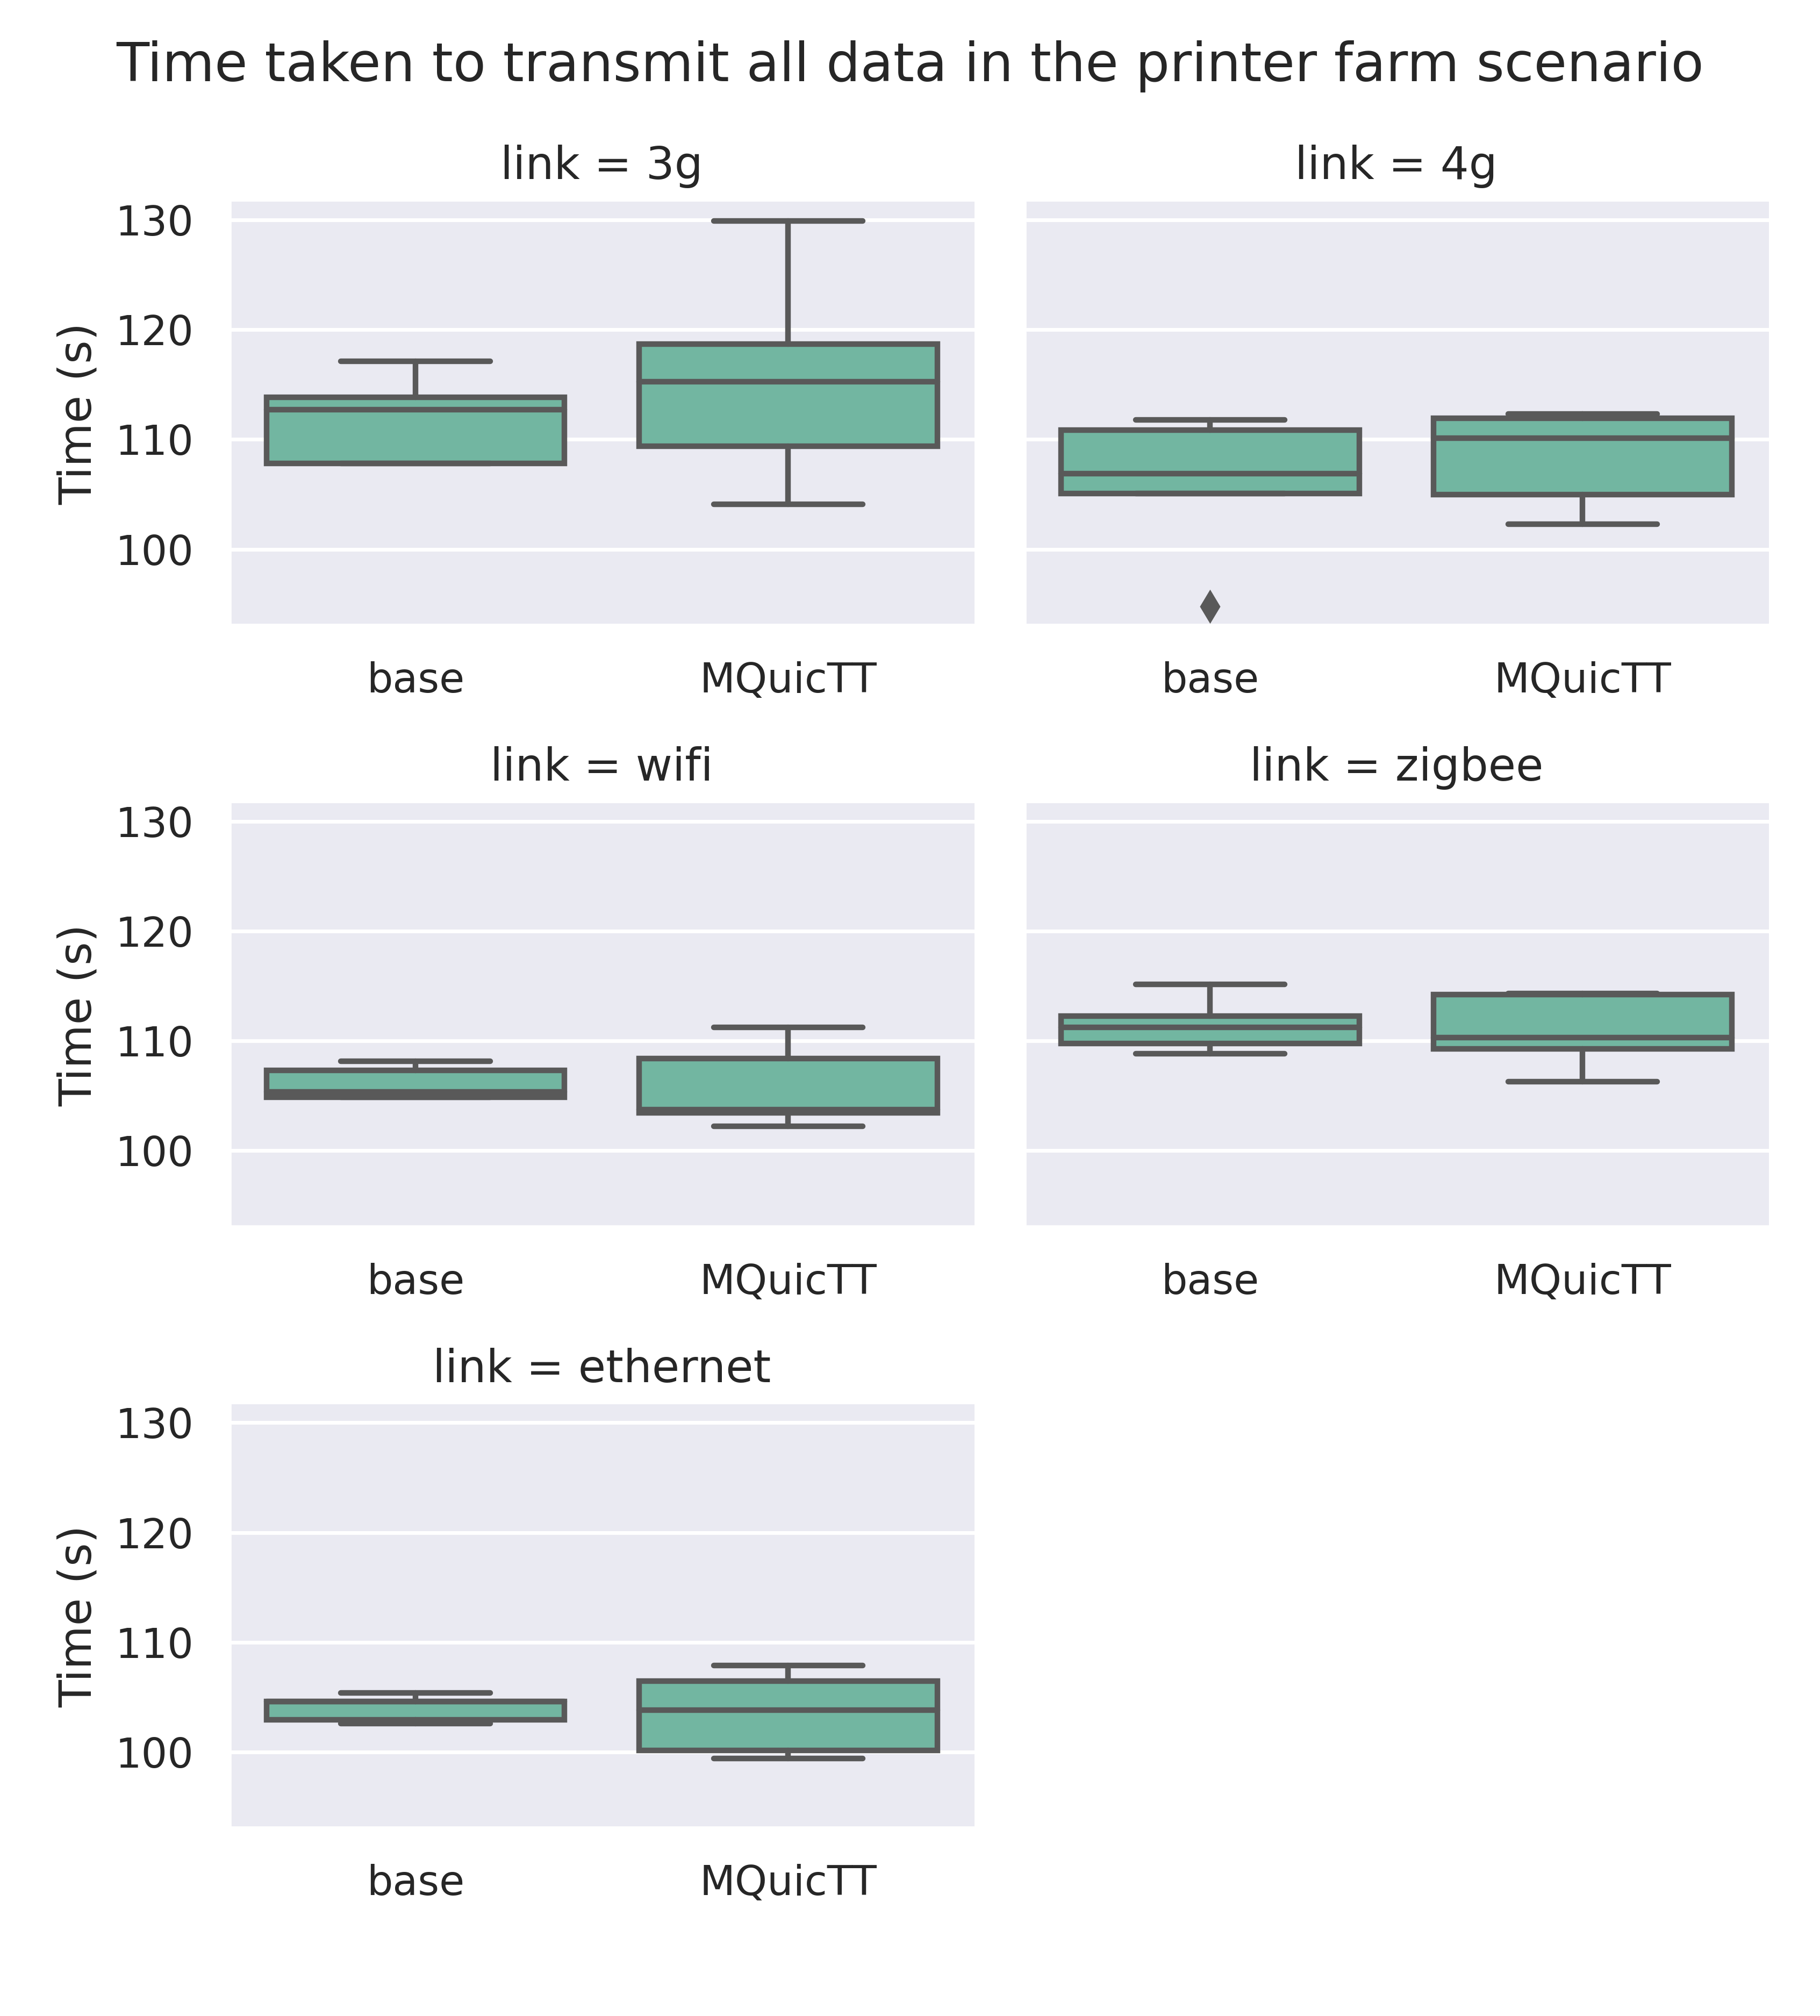
\includegraphics[width=1\linewidth]{images/analysis_comm_time_farm.png}
    \caption{The time it took for the implementations to transmit the MQTT messages in the printer farm scenario.
        The time for each plot is shown in seconds.
        We can see that the results are similar to the IoT home scenario.}
    \label{fig:comm_time_farm}
\end{figure}

Hence, we now look at Figure~\ref{fig:comm_time_synth} which shows the results for the synthetic scenario.
That is, the scenario with extreme packet loss.
The results of this scenario echo the previous ones.
$MQuicTT$ performs as well as the base $rumqtt$ with the results for ethernet showing a performance increase in favour of the QUIC implementation.
Notably, we can see that in this scenario, both implementations experienced greater variance in measurements.
Overall, $MQuicTT$ performed as well as the base implementation in each scenario, however, it also presented no performance improvement.

\begin{figure}
    \centering
    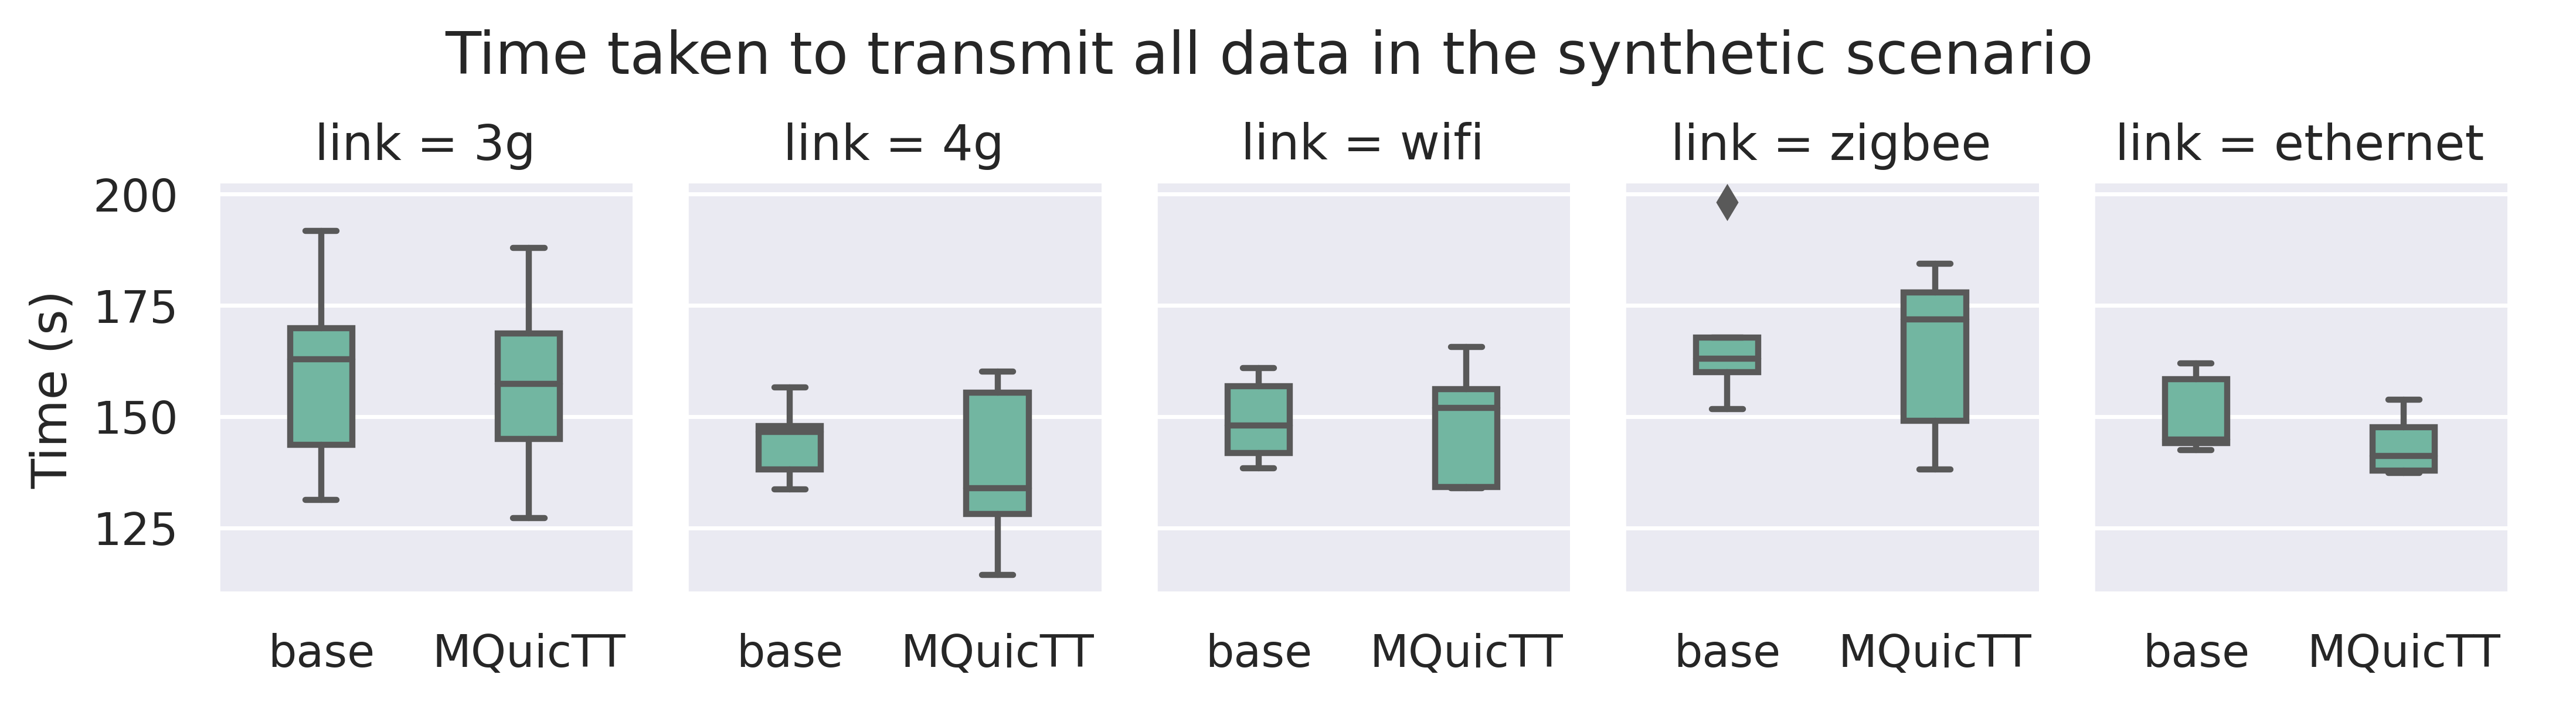
\includegraphics[width=1\linewidth]{images/analysis_comm_time_synth.png}
    \caption{The time it took for the implementations to transmit the MQTT messages in the printer farm scenario.
        The time for each plot is shown in seconds.}
    \label{fig:comm_time_synth}
\end{figure}